% !TeX program = pdflatex
\documentclass[research]{fcs}

\title{Profiling Sparse-Index Gradient Accumulation in Backpropagation: A PyTorch CUDA Study of Embedding, Index-Add, and Scatter-Add Paths}
\shorttitle{Sparse-Index Gradient Accumulation in PyTorch CUDA}

\author[1,+]{Marko Mihajlović}
\address[1]{Singidunum University, PhD Student, Belgrade, Serbia}
% Corresponding author: Marko Mihajlović
% TODO: Add ORCID 0009-0006-7979-0341 if the selected FCS submission workflow supports it.
\corremail{marko.mihajlovic.23@singimail.rs}

\fcssetup{
  received = {2026},
  accepted = {2026},
  article-id = {1},
  first-page = {1},
}

\begin{abstract}
Sparse-index gradient accumulation is a recurring operation in backpropagation for embedding-heavy and sparse-feature AI training workloads. Although high-level tensor APIs may express related accumulation semantics, their CUDA execution paths can differ substantially in practice. This paper presents a controlled empirical study of three standard PyTorch CUDA paths for sparse-index accumulation: \texttt{index\_add}, \texttt{scatter\_add}, and \texttt{Embedding.backward}. The study uses a calibrated benchmark protocol with correctness validation, matched workload configurations, CUDA-event timing, a practical-margin rule for winner classification, and representative profiler-based attribution.

The results show that the fastest API path is workload- and stack-dependent. In the matched benchmark phase, the local GTX1650Ti stack most often favored \texttt{Embedding.backward}, whereas the T4 stacks most often favored \texttt{scatter\_add}. Representative profiler evidence further shows that the three APIs dispatch to distinct CUDA kernel compositions: \texttt{index\_add} is dominated by indexed accumulation kernels, \texttt{scatter\_add} by scatter/gather-style accumulation kernels, and \texttt{Embedding.backward} by a multi-kernel backward path that includes accumulation and sorting or segmentation-related components. Strong representative reversals confirm that high-level API similarity does not guarantee equivalent performance behavior.

These findings indicate that sparse-index gradient accumulation should be treated as a workload- and software/hardware-stack-dependent systems problem rather than as a purely semantic API choice. The study does not claim a universal fastest API or isolated hardware causality; instead, it provides a reproducible characterization of standard PyTorch CUDA paths under controlled sparse-gradient accumulation workloads.
\end{abstract}
\keywords{Sparse gradients; Sparse-index accumulation; Backpropagation; PyTorch; CUDA; Embedding backward; Index add; Scatter add; AI model training}

\begin{document}

\section{Introduction}

Modern AI training workloads are not composed only of dense matrix multiplication, convolution, or attention kernels. Many practical models also contain sparse or irregular components whose performance is shaped by index distributions, memory access patterns, and reduction behavior. This is especially visible in recommendation and sparse-feature models, where large embedding tables are used to represent categorical identifiers and where training efficiency depends on both dense neural-network computation and memory-intensive embedding operations \cite{gupta2020architectural,acun2021training}. Recent work on large-scale embedding optimization further shows that embedding access patterns, repeated indices, and gradient processing remain important systems-level concerns in recommendation-model training \cite{liu2024embark}.

A central operation in such workloads is sparse-index gradient accumulation during backpropagation. In the forward pass, indexed operations such as embedding lookup gather rows from a parameter table. In the backward pass, gradients associated with those indexed rows must be routed back and accumulated into the corresponding parameter-gradient structure. When the same index appears multiple times in a batch, several gradient contributions target the same destination row. This creates an indexed aggregation problem rather than a purely dense tensor operation. The cost of this aggregation can depend on the number of rows, number of indices, feature dimension, index skew, duplicate-index frequency, memory layout, and the CUDA execution path selected by the framework.

PyTorch exposes several high-level APIs that can express related accumulation-style behavior. The \texttt{torch.nn.Embedding} module provides a standard embedding-table abstraction and supports sparse gradients with respect to embedding weights in selected configurations \cite{pytorchStableEmbedding}. Tensor-level APIs such as \texttt{index\_add\_}, \texttt{scatter\_add}, and \texttt{scatter\_add\_} also describe indexed accumulation or scatter-add semantics \cite{pytorchStableIndexAdd,pytorchStableScatterAdd,pytorchStableTensorScatterAdd}. From the perspective of a model developer, these APIs may appear to represent closely related ways of accumulating indexed values. However, high-level semantic similarity does not imply that the same CUDA kernels, memory behavior, or performance characteristics are used internally.

This distinction matters because GPU execution is asynchronous, parallel, and sensitive to reduction order, memory access, and synchronization behavior. PyTorch documentation notes that CUDA execution is asynchronous relative to the CPU, which makes synchronization-aware timing necessary for accurate measurement \cite{pytorchStableCUDASemantics}. PyTorch also documents nondeterminism concerns for selected CUDA operations and reproducibility settings \cite{pytorchStableReproducibility}. At the same time, CUDA event timing and profiler-based kernel attribution provide practical tools for separating clean latency measurements from diagnostic execution-path analysis \cite{nvidiaCUDAEvents,pytorchStableProfiler,nvidiaNsightCompute}. These properties make sparse-index accumulation a suitable target for controlled benchmarking and profiling.

Prior work has studied sparse GPU kernels, irregular graph and sparse-matrix workloads, recommendation-system architectures, and large-scale embedding optimization \cite{gale2020sparse,wang2016gunrock,huang2020gespmm,gupta2020architectural,acun2021training,liu2024embark}. These studies establish that sparse and irregular workloads are important and that their performance depends on memory behavior, data distribution, and execution strategy. However, they do not directly answer a narrower practical question faced by PyTorch users: how do standard PyTorch CUDA paths such as \texttt{index\_add}, \texttt{scatter\_add}, and \texttt{Embedding.backward} compare under matched sparse-index gradient accumulation workloads?

This paper addresses that question through a controlled empirical study of sparse-index gradient accumulation during backpropagation-style computation. The study evaluates standard PyTorch CUDA paths rather than custom CUDA kernels. It first calibrates the benchmark protocol and validation rules, then performs a matched grid-level timing comparison, and finally uses representative profiler runs to relate timing behavior to CUDA execution paths. The goal is not to identify a universally fastest API, but to characterize when and how the relative behavior of these APIs changes across workloads and execution stacks.

The contributions of the paper are fourfold. First, it defines a controlled benchmark protocol for comparing standard PyTorch CUDA accumulation paths under matched sparse-index workloads. Second, it provides grid-level timing evidence for \texttt{index\_add}, \texttt{scatter\_add}, and \texttt{Embedding.backward} across workload configurations relevant to sparse-gradient accumulation. Third, it links representative timing differences to CUDA profiler evidence, showing that the APIs dispatch to distinct execution paths rather than merely different surface syntax. Fourth, it discusses the implications of these findings for embedding-heavy AI training workloads, while explicitly separating stack-level empirical observations from universal API rankings or isolated hardware-causal claims.

The rest of the paper is organized as follows. Section~\ref{sec:background-related-work} reviews sparse operations in AI training, embedding-heavy workloads, indexed accumulation APIs, CUDA execution behavior, and related profiling methodology. Section~\ref{sec:methodology} describes the benchmark scope, workload design, correctness validation, timing methodology, profiling methodology, and cross-environment comparison. Section~\ref{sec:results-analysis} presents the calibrated benchmark results, matched Phase 2 timing evidence, representative Phase 3 profiler results, and result-level discussion. Section~\ref{sec:general-discussion} discusses significance, practical implications, limitations, generalizability, and future work. Section~\ref{sec:conclusion} concludes the paper.
\section{Background and Related Work}
\label{sec:background-related-work}

Sparse and irregular computation has become an important systems issue in modern machine learning workloads. While many neural-network accelerators and GPU software stacks are highly optimized for dense tensor operations, sparse workloads introduce indirect memory access, data-dependent work distribution, and irregular reduction patterns. Prior work on sparse GPU kernels shows that sparsity does not automatically translate into speedup; performance depends on workload structure, memory access, load balance, and the ability of the implementation to exploit the sparsity pattern efficiently \cite{gale2020sparse}. Related GPU graph-processing and sparse-matrix work has similarly shown that irregular active sets, sparse aggregation, and uncoalesced memory accesses require specialized runtime or kernel-level strategies rather than simple reuse of dense-compute assumptions \cite{wang2016gunrock,huang2020gespmm}.

These issues are especially relevant in AI training workloads that use embedding tables and sparse categorical features. Production recommendation models combine memory-intensive embedding components with dense neural-network layers, and their performance behavior differs from conventional dense CNN-style or MLP-style workloads \cite{gupta2020architectural}. Training such models adds further complexity because the backward pass must update or accumulate gradients for the embedding rows referenced by the training batch. System-level studies of recommendation training have shown that embedding tables, sparse features, model configuration, and data placement can materially affect training efficiency at scale \cite{acun2021training}. More recent work on embedding optimization for large-scale recommendation training also emphasizes that repeated and skewed embedding accesses can make embedding-gradient processing an important optimization target \cite{liu2024embark}.

At the operator level, embedding backward computation can be viewed as a form of indexed gradient accumulation. During the forward pass, an embedding layer maps integer identifiers to dense vectors. During the backward pass, gradients associated with repeated identifiers must be routed back to the corresponding parameter rows and accumulated. PyTorch exposes this layer through \texttt{torch.nn.Embedding}, whose documentation defines it as a lookup table and notes that the gradient with respect to the embedding weight can optionally be represented sparsely when \texttt{sparse=True} \cite{pytorchStableEmbedding}. This public API behavior motivates treating \texttt{Embedding.backward} as a realistic training-related accumulation path rather than only as a synthetic tensor primitive.

General tensor APIs can express related indexed accumulation patterns. PyTorch documents \texttt{index\_add\_} as an operation that accumulates selected slices from a source tensor into a destination tensor according to a one-dimensional index, and it explicitly warns that CUDA execution may be nondeterministic \cite{pytorchStableIndexAdd}. PyTorch also documents \texttt{scatter\_add} as the out-of-place form of \texttt{Tensor.scatter\_add\_}, while \texttt{scatter\_add\_} adds values into destinations selected by an index tensor and also carries CUDA nondeterminism caveats \cite{pytorchStableScatterAdd,pytorchStableTensorScatterAdd}. These APIs are therefore natural candidates for implementing or approximating sparse-index gradient accumulation, but their public semantics do not imply that they dispatch to the same CUDA kernels or have the same performance behavior.

The relevance of nondeterminism follows from the reduction structure of indexed accumulation. When several source elements contribute to the same destination row, the implementation must combine those contributions. On GPUs, this often requires atomic updates or staged reduction strategies, and the order of floating-point additions may vary across parallel executions. The CUDA programming guide defines atomic operations as read-modify-write operations with specific memory and scope semantics \cite{nvidia2026cudaguide}. PyTorch's reproducibility documentation likewise cautions that complete reproducibility is not guaranteed across releases, platforms, and devices, and that deterministic alternatives may change execution behavior or reject unsupported operations \cite{pytorchStableReproducibility}. For this reason, sparse-index accumulation must be studied with both correctness tolerance and performance behavior in mind.

The broader GPU literature also supports the need to treat indexed aggregation as a workload-dependent systems problem. Graph-processing frameworks such as Gunrock are designed around irregular GPU workloads and data-centric parallelism rather than dense regular computation \cite{wang2016gunrock}. Sparse matrix multiplication work for graph-neural-network workloads similarly shows that data reuse, memory access, and sparse representation choices can dominate practical performance \cite{huang2020gespmm}. Although these systems do not directly study PyTorch \texttt{index\_add}, \texttt{scatter\_add}, or \texttt{Embedding.backward}, they provide important background for why irregular indexed aggregation may behave differently across input distributions and execution stacks.

Empirical evaluation of such operations requires careful GPU timing methodology. CUDA execution in PyTorch is asynchronous relative to the CPU, so host-side timing without synchronization can measure dispatch overhead rather than device execution time \cite{pytorchStableCUDASemantics}. PyTorch's benchmarking and profiler documentation supports repeated measurements, warmup, synchronization-aware measurement, and explicit separation between clean timing and profiler-instrumented analysis \cite{pytorchBenchmarkRecipe,pytorchStableProfiler,pytorchProfilerRecipe}. NVIDIA's CUDA event documentation provides the lower-level basis for event-based elapsed-time measurement, while NVIDIA profiling documentation emphasizes that metric collection and profiling can introduce overhead and should be interpreted as diagnostic rather than identical to uninstrumented latency measurement \cite{nvidiaCUDAEvents,nvidiaNsightCompute}.

Existing work therefore covers several adjacent areas: sparse GPU kernels, irregular graph aggregation, recommendation-system architectures, large-scale embedding training, PyTorch API semantics, CUDA atomics, nondeterminism, and profiling methodology. However, these strands do not by themselves provide a controlled empirical comparison of the standard PyTorch CUDA paths for \texttt{index\_add}, \texttt{scatter\_add}, and \texttt{Embedding.backward} under matched sparse-index gradient accumulation workloads. Prior work often focuses either on complete recommender systems, specialized embedding-training systems, custom sparse kernels, graph runtimes, or general GPU profiling. This leaves room for a narrower empirical characterization of how commonly available PyTorch APIs behave when they are used to express related backpropagation-style sparse-index accumulation patterns.

The gap addressed by this paper is therefore not the novelty of indexed reduction itself. Indexed accumulation, embedding gradients, sparse GPU kernels, and recommendation workloads are all well-established research areas. The contribution is instead a controlled, version- and stack-aware characterization of standard PyTorch CUDA execution paths for sparse-index gradient accumulation. By comparing \texttt{index\_add}, \texttt{scatter\_add}, and \texttt{Embedding.backward} under matched workloads and then linking timing behavior to profiler evidence, the study aims to clarify when high-level API similarity does and does not correspond to similar CUDA execution behavior.
\section{Methodology}
\label{sec:methodology}

\subsection{Study Scope}

This study investigates sparse-index gradient accumulation patterns that arise during the backpropagation phase of AI model training. The focus is on workloads in which many indexed source vectors contribute to a dense gradient-like output, a pattern that is common in embedding tables, recommender-style models, negative sampling, graph workloads, and other training settings where sparse index references are accumulated during the backward pass.

The study is intentionally scoped to standard PyTorch CUDA execution paths rather than custom CUDA kernels. The goal is not to design a new accumulation primitive, but to characterize how widely available PyTorch APIs behave under controlled sparse-index accumulation workloads. In particular, the experiments examine whether API-level alternatives that express similar accumulation-style computations can exhibit different timing behavior and different CUDA execution paths.

The study does not benchmark full model training, end-to-end training throughput, dense matrix multiplication, convolution, attention, optimizer performance, data loading, or distributed training. These components are outside the scope because they would introduce additional sources of variation that are not necessary for isolating the sparse-index accumulation behavior studied here. Instead, the experimental design separates a grid-level timing phase from a representative profiling phase. The grid-level phase provides the main matched timing evidence, while the profiling phase provides execution-path attribution for selected representative cases.

\subsection{Benchmarked Operations}

The comparison centers on three PyTorch CUDA operations or operation paths:

\begin{itemize}[leftmargin=*]
    \item \texttt{index\_add}, which accumulates source rows into a dense output according to an index tensor;
    \item \texttt{scatter\_add}, which expresses an indexed accumulation pattern through scatter-style updates;
    \item \texttt{Embedding.backward}, which represents the backward path of a PyTorch embedding table and therefore provides a realistic training-related sparse-gradient accumulation path.
\end{itemize}

These operations are conceptually related because each can be used to represent sparse-index accumulation into a dense gradient-like tensor under controlled workload construction. However, the study does not assume that they are universally equivalent in all PyTorch contexts or all mathematical formulations. Instead, they are compared under matched accumulation-style workloads in which the input shapes, index distributions, and output dimensions are controlled.

The inclusion of \texttt{Embedding.backward} is important because embedding tables are a common source of sparse gradient accumulation during backpropagation. Unlike the direct accumulation APIs, the embedding backward path may involve specialized internal kernels and additional framework-level logic. Comparing it with \texttt{index\_add} and \texttt{scatter\_add} therefore helps distinguish API-level similarity from actual CUDA execution behavior.

\subsection{Workload Design}

Workloads are parameterized by the number of output rows, the number of indexed source entries, the feature dimension, and the distribution of index values. The main workload parameters are:

\begin{itemize}[leftmargin=*]
    \item \texttt{rows}: the number of rows in the dense output or embedding table;
    \item \texttt{indices}: the number of indexed source entries accumulated during the operation;
    \item \texttt{dim}: the feature dimension of each row;
    \item \texttt{distribution}: the statistical distribution used to generate index references;
    \item \texttt{workload\_draw}: the workload draw identifier used to construct matched cases;
    \item \texttt{zipf\_mode}: the mode used for Zipf-distributed workloads;
    \item \texttt{row\_layout}: the layout of rows in the generated workload;
    \item \texttt{index\_order}: the order of generated indices;
    \item \texttt{cache\_mode}: whether the workload is evaluated under the selected cache condition.
\end{itemize}

The workload distributions include uniform, Zipf, and hotspot-style index patterns. Uniform workloads provide a baseline in which index references are more evenly distributed across rows. Zipf and hotspot workloads introduce skew, duplicate references, and hot rows. These skewed cases are important because duplicate indices can change the cost of accumulation and can expose differences between accumulation implementations.

The broader timing phase evaluates matched configurations across a larger workload grid. The profiling phase uses a smaller set of representative cases selected to expose the CUDA execution paths underlying the observed API behavior. This separation avoids relying on profiler-instrumented runs as the primary timing evidence while still allowing the study to inspect representative kernel-level composition.

\subsection{Correctness Validation}

Correctness validation is performed before timing or profiling results are accepted into the analysis. This is necessary because timing comparisons are meaningful only when the operations compute the intended accumulation result under the same workload configuration.

For each accepted configuration, the benchmark checks that the compared operation produces numerically valid output relative to the reference accumulation behavior used by the experiment. Rows with failed correctness checks or failed execution status are excluded from paired winner claims. This rule applies both to the broader timing phase and to the representative profiling phase.

The correctness procedure is especially important for sparse-index workloads because repeated indices, skewed distributions, and different internal execution paths may change the order of floating-point accumulation. The validation therefore uses tolerance-based numerical checks rather than assuming bitwise equality in every case. This preserves the focus on computational equivalence within a practical numerical tolerance while allowing the study to compare different CUDA-backed execution paths.

\subsection{Timing Methodology}

The primary timing evidence comes from CUDA-event measurements over matched workload configurations. For each configuration, the selected operations are compared within the same workload setting. The timing analysis uses median latency as the main summary statistic, because medians are less sensitive to occasional runtime outliers than single measurements or means alone.

A practical margin threshold is used to distinguish decisive timing differences from near-ties. Specifically, when the runner-up operation is more than 5\% slower than the fastest operation for a matched configuration, the fastest operation is treated as the practical winner for that case. If the margin does not exceed this threshold, the case is retained but interpreted as a near-tie rather than strong evidence of a meaningful performance difference.

The broader matched timing phase is the main source of grid-level performance evidence. The representative profiling phase also records event timings for the selected cases, but those timings are used primarily to relate profiled cases to the broader benchmark behavior. They are not treated as a replacement for the broader timing grid because the profiling subset is smaller and uses a fixed representative design.

The timing methodology distinguishes between direct operation timing and profiler-derived quantities. CUDA-event medians are used for operation-level timing comparisons, while profiler-derived CUDA totals are used for attribution and diagnostic interpretation. These two measurement sources are not interchangeable because profiling introduces instrumentation, synchronization, and event collection overhead.

\subsection{Profiling Methodology}

The profiling phase is designed to identify the CUDA execution paths associated with the selected PyTorch APIs. It uses representative workloads from the same accumulation setting and records profiler outputs for each case-operation pair. The relevant profiling artifacts include:

\begin{itemize}[leftmargin=*]
    \item \texttt{profile\_cases.csv}, which records case-level operation status, timing summaries, profiler attribution fields, and diagnostic flags;
    \item \texttt{case\_winners.csv}, which records the fastest operation and runner-up for each representative case;
    \item \texttt{profile\_events\_caseXX\_operation.csv}, which records full profiler event rows when available;
    \item \texttt{profile\_top\_cuda\_caseXX\_operation.csv}, which records the top CUDA events for each profiled operation.
\end{itemize}

Full CUDA event files are preferred over top-event summaries when computing kernel-category shares. User annotations and enclosing profiling ranges are excluded from category-share calculations so that the resulting summaries reflect CUDA device work rather than inclusive annotation ranges. When only top-event summaries are available, the analysis treats them as truncated attribution evidence rather than full-profile composition.

The profiler events are grouped into conservative name-based categories. The categories used for interpretation are:

\begin{itemize}[leftmargin=*]
    \item \texttt{index\_add\_accumulate}, for CUDA kernels associated with indexed reduction through the \texttt{index\_add} path;
    \item \texttt{scatter\_add\_accumulate}, for CUDA kernels associated with scatter/gather reduction paths;
    \item \texttt{embedding\_accumulate}, for embedding backward accumulation kernels such as gradient-weight computation and scatter-style accumulation inside the embedding backward path;
    \item \texttt{sort\_scan\_unique}, for sort, scan, and unique-related kernels that appear in the embedding backward path;
    \item \texttt{zero\_fill\_memset}, for initialization and zero-fill kernels;
    \item \texttt{arange\_index\_setup}, for index setup kernels such as range construction;
    \item \texttt{other}, for CUDA events not captured by the preceding categories.
\end{itemize}

These categories are used for execution-path attribution, not for proving low-level hardware causality. They are based on observed kernel and operator names, and therefore depend on the PyTorch and CUDA software stack used in each environment. The category summaries are intended to show whether the three PyTorch APIs exercise distinct CUDA paths under the profiled workloads.

The profiling phase also computes a GPU-busy proxy by comparing profiler-derived CUDA kernel time with the unprofiled CUDA-event timing for the same case. This proxy is used only as a warning signal for possible host overhead. It is not a hardware utilization counter and is not interpreted as a direct measurement of GPU occupancy or saturation.

\subsection{Cross-Environment Comparison}

The study compares two execution environments: a local GTX1650Ti stack and a Colab Tesla T4 stack. These environments differ not only in GPU model, but also in operating system, runtime conditions, PyTorch version, CUDA version, and hosted execution context. Therefore, the comparison is interpreted as a stack-level comparison rather than an isolated hardware-causal experiment.

The cross-environment analysis is performed in two stages. First, the broader matched timing analysis compares winner counts, practical-margin winners, and relative speedups across the matched workload grid. Second, the representative profiling analysis compares selected cases across the two environments and relates them back to the matched timing grid.

The comparison artifacts serve distinct purposes. The \texttt{phase3\_case\_comparison.csv} table records the representative case-level winners, margins, host-warning flags, timing-stability flags, index-hash pairing status, and winner-relation categories. The \texttt{phase3\_phase2\_case\_join.csv} table links the representative profiling cases back to the broader matched Phase 2 grid, allowing the analysis to determine whether a profiled case is present in the broader timing evidence. The \texttt{phase3\_claim\_checks.csv} table records evidence gates used to determine which paper-level claims are supported by the available data.

Workload pairing is checked through parameter matching and index hashes where available. Matching index hashes provide stronger evidence that the same index draw is being compared across environments. Source tensor hashes may differ across environments due to random number generation and software-stack differences, so source-hash mismatches are treated as informational rather than automatic failures.

\subsection{Threats to Validity}

Several threats to validity limit the interpretation of this study.

First, the profiling phase uses a representative subset rather than the full workload grid. The representative cases are useful for execution-path attribution, but they are not sufficient to establish grid-wide frequencies or statistical performance distributions on their own. For this reason, the broader matched timing phase remains the main source of performance evidence.

Second, the representative profiling phase uses a fixed operation order and a limited per-case measurement design. This makes the profiler outputs easier to inspect and compare, but it also means that the profiling subset should not be treated as a randomized timing experiment.

Third, profiler overhead can perturb execution. Profiler-derived CUDA totals are therefore used for attribution and diagnostic interpretation rather than as the primary timing metric. CUDA-event medians remain the main basis for operation-level timing comparisons.

Fourth, the GPU-busy proxy is not a hardware utilization counter. Values derived from profiler events can be affected by synchronization, instrumentation overhead, and differences between profiled and unprofiled timing conditions. A low value is treated only as a warning signal for possible host overhead.

Fifth, the two environments differ in multiple dimensions, including GPU model, operating system, PyTorch version, CUDA version, and hosted runtime conditions. Consequently, the study does not make isolated hardware-causal claims. Observed differences are attributed to the combined hardware/software stack and workload configuration.

Sixth, the study does not use Nsight Compute counters, hardware occupancy metrics, memory-transaction counters, or warp-level profiling. The kernel attribution is based on PyTorch profiler event names and CUDA event durations, which provide useful execution-path evidence but do not fully explain microarchitectural causes.

Seventh, the study does not benchmark full training loops or end-to-end model convergence. The results therefore apply to controlled sparse-index accumulation behavior rather than complete model training throughput.

Finally, the study does not compare against custom CUDA implementations. This is intentional because the research question concerns the behavior of standard PyTorch CUDA APIs available to practitioners, but it also means that the results should not be interpreted as the best possible performance attainable for sparse-index gradient accumulation.
\section{Results and Analysis}
\label{sec:results-analysis}

This section presents the experimental evidence in the same order in which the benchmark design was developed and validated. The first phase establishes the baseline behavior of the benchmark and verifies the methodological assumptions needed for fair comparison. The second phase provides the main matched grid-level timing evidence across the selected PyTorch CUDA accumulation paths. The third phase complements the timing results with profiler evidence for representative cases, allowing the observed performance differences to be related to the CUDA execution paths used by each API.

The analysis therefore separates three roles. Phase 1 is treated as a calibration and validation phase, because its purpose is to justify the final benchmark protocol rather than to provide the main paper-level performance claim. Phase 2 is treated as the primary timing phase, because it compares the selected operations across a matched workload grid. Phase 3 is treated as the attribution phase, because it explains selected Phase 2 patterns through CUDA profiler evidence. This separation is important because the study does not rely on a single timing table or a single profiler run; instead, the final interpretation combines protocol validation, matched timing, and representative execution-path analysis.

\subsection{Phase 1 Baseline Calibration and Methodological Checks}

Phase 1 was used to establish a reliable benchmark protocol before the final matched comparison was performed. At this stage, the purpose was not to select a final winning API, but to identify which timing scope, workload construction, and validation rules were appropriate for comparing sparse-index accumulation paths during backpropagation-style computation. The early benchmark runs helped separate experimental configurations that were useful for methodological diagnosis from configurations that were suitable for final matched comparison.

A central outcome of this phase was the need to define a fair dense-gradient accumulation scope. For direct accumulation APIs such as \texttt{index\_add} and \texttt{scatter\_add}, timing only the update kernel without accounting for the dense output buffer would not match the practical cost of producing a dense gradient-like result. Phase 1 therefore motivated the final timing scope in which dense output allocation or zero initialization is included where required by the operation design. This made the later comparison closer to the practical cost of producing the accumulated output, rather than measuring only an isolated kernel fragment.

Phase 1 also clarified the role of \texttt{Embedding.backward}. The embedding backward path is not simply a syntactic variant of \texttt{index\_add} or \texttt{scatter\_add}. It is a framework-level backward path with its own internal dispatch behavior and memory-management assumptions. For this reason, the final protocol treats \texttt{Embedding.backward} as a realistic training-related path rather than forcing it into the exact same implementation scope as the direct accumulation APIs. This distinction is important because the paper studies the behavior of standard PyTorch CUDA paths as they are exposed to practitioners, not an artificially rewritten version of each operation.

The first phase further established the importance of correctness validation before timing interpretation. Sparse-index accumulation workloads often contain repeated indices, and different execution paths may accumulate floating-point values in different orders. As a result, bitwise equality is not an appropriate universal requirement for accepting a timing row. Phase 1 therefore motivated the use of tolerance-based numerical validation and the exclusion of failed correctness rows from paired performance claims. This validation gate was then carried forward into the later matched benchmark and profiler phases.

Another methodological result from Phase 1 was the decision to distinguish decisive timing differences from near-ties. Small differences between operation medians can occur because of normal runtime variability, measurement noise, or cache and scheduling effects. Treating every raw minimum as a meaningful winner would overstate the evidence. The later analysis therefore applies a practical margin rule, where a winner is treated as decisive only when the runner-up is more than 5\% slower. Cases below this threshold are retained in the dataset but interpreted as near-ties rather than strong performance evidence.

Phase 1 also informed the workload design used in the final study. The benchmark needed to include not only uniform index distributions, but also skewed patterns such as Zipf and hotspot distributions. These distributions are relevant because duplicate indices and hot rows can change the behavior of accumulation kernels. The preliminary checks therefore motivated a workload design that varies row count, number of indices, feature dimension, distribution type, index ordering, and cache-related conditions. This broader design was necessary to avoid drawing conclusions from a single synthetic shape or a single index distribution.

The outcome of Phase 1 was therefore a calibrated experimental protocol for the final comparison. The final protocol uses matched workloads, correctness-gated rows, median CUDA-event timing, a practical-margin rule for winner classification, and a distinction between grid-level timing evidence and profiler-based attribution. Phase 1 is not presented as the main evidence for the paper's performance claims; instead, it explains why the subsequent Phase 2 and Phase 3 analyses are structured as matched timing and representative profiling phases.

\subsection{Matched Phase 2 Benchmark Results}

The matched Phase 2 benchmark provides the main grid-level evidence for the study. In this phase, the three selected PyTorch accumulation paths were compared under shared workload configurations, using the same rows, index counts, feature dimensions, distribution types, layout settings, and cache conditions within each matched case. The purpose of this phase was to determine whether the fastest API path is stable across environments or whether it changes with the workload and software/hardware stack.

Table~\ref{tab:phase2-winner-counts} summarizes the practical-margin winner counts across the matched Phase 2 grid. The local GTX1650Ti environment favored \texttt{embedding} most often, with 96 decisive wins out of 162 matched configurations. The same environment selected \texttt{index\_add} in 60 configurations, while \texttt{scatter\_add} did not obtain a decisive win under the practical-margin rule. Six configurations were classified as ties. In contrast, the T4 environment favored \texttt{scatter\_add} most often, with 92 decisive wins out of 162 configurations. The repeated T4 run reproduced the same qualitative pattern, with \texttt{scatter\_add} selected in 93 out of 162 configurations.

% Source summary: sparse-gradient/phase2_analysis_v2/ and matched Phase 2 analysis.
\begin{table}[tbp]
\centering
\small
\caption{Matched Phase 2 winner counts for the three primary accumulation paths under the 5\% practical-margin rule.}
\label{tab:phase2-winner-counts}
\resizebox{\linewidth}{!}{%
\begin{tabular}{lrrrrrr}
\toprule
Environment & \texttt{index\_add} & \texttt{scatter\_add} & \texttt{embedding} & Tie & Total matched configurations & Most frequent decisive API \\
\midrule
GTX1650Ti & 60 & 0 & 96 & 6 & 162 & \texttt{embedding} \\
T4 & 5 & 92 & 25 & 40 & 162 & \texttt{scatter\_add} \\
T4\_repeat & 1 & 93 & 27 & 41 & 162 & \texttt{scatter\_add} \\
\bottomrule
\end{tabular}
}%
\end{table}


The Phase 2 results therefore indicate that there is no single universally dominant API path across the studied environments. The local stack most often favors the embedding backward path, whereas the T4 stacks most often favor the scatter-add path. This difference is not interpreted as an isolated GPU-hardware effect, because the environments differ in GPU model, operating system, PyTorch version, CUDA version, and hosted execution conditions. Instead, the result motivates a stack-level interpretation: the relative cost of the available PyTorch CUDA paths depends on the combination of workload structure and execution environment.

The practical-margin rule is important for interpreting these counts. Configurations in which the fastest and runner-up operations differ by less than the selected 5\% threshold are retained as near-ties rather than treated as decisive evidence. This prevents small timing differences from being overinterpreted as meaningful API-level superiority. Consequently, the Phase 2 result should be read as a matched practical-performance characterization, not as a statistical proof of universal API ranking.

\subsection{Representative Phase 3 Profiling Results}

Phase 3 complements the Phase 2 timing grid by profiling a representative subset of six workload cases. The purpose of this phase is not to replace the broader timing evidence, but to inspect the CUDA execution paths associated with the selected PyTorch APIs. Each representative case is evaluated for \texttt{index\_add}, \texttt{scatter\_add}, and \texttt{Embedding.backward}, resulting in 18 profiled case-operation rows per environment.

The profiling outputs passed the basic execution and correctness checks in both environments. Each environment produced 18 successful case-operation rows, with no failed execution status and no correctness failures. CUDA kernel attribution was available for all 18 profiled rows in both environments. The T4 environment contained one host-overhead warning, associated with the \texttt{embedding} operation in case04; this case is therefore interpreted cautiously when making GPU-clean attribution claims.

Fig.~\ref{fig:phase3-median-ms} shows the representative Phase 3 event-timing medians by case and operation. These values are useful for relating the profiled subset to the broader timing behavior, but they are not treated as a replacement for the matched Phase 2 grid. The profiled subset uses a smaller number of cases and is primarily designed for attribution rather than grid-level performance counting.

\begin{figure}[tbp]
\centering
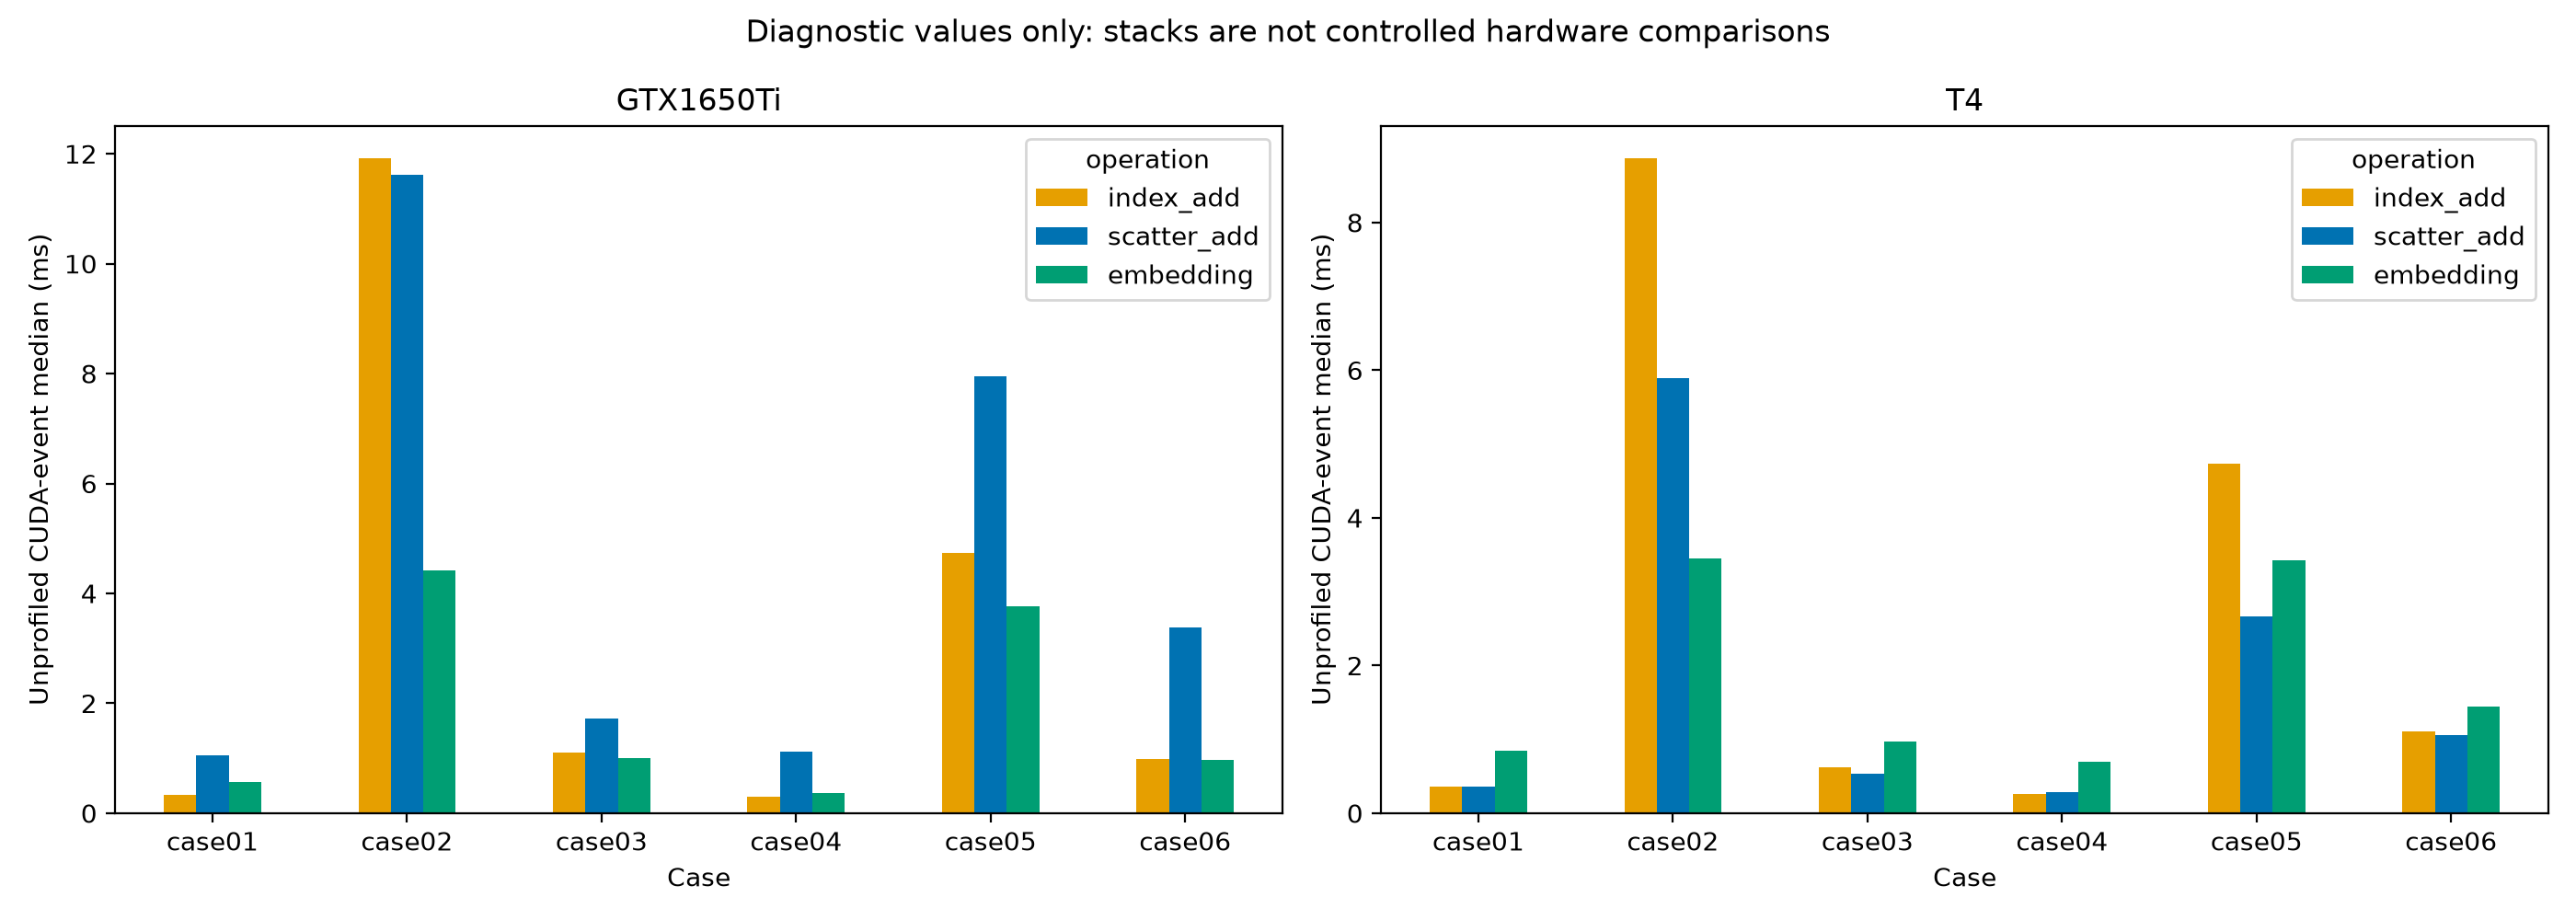
\includegraphics[width=0.80\linewidth]{figures/phase3_median_ms_by_case_operation.png}
\caption{Phase 3 median CUDA-event timing by representative case and operation. These timings describe the profiled subset and are interpreted together with the broader matched Phase 2 grid.}
\label{fig:phase3-median-ms}
\end{figure}

Fig.~\ref{fig:phase3-gpu-busy} summarizes the profiler-derived GPU-busy proxy. The proxy is used only as a warning signal for possible host overhead, not as a hardware utilization counter. Most profiled case-operation rows have high proxy values, supporting their use for execution-path attribution. The main exception is the T4 \texttt{embedding} row in case04, which is flagged and therefore not used as a clean GPU-bound claim.

\begin{figure}[tbp]
\centering
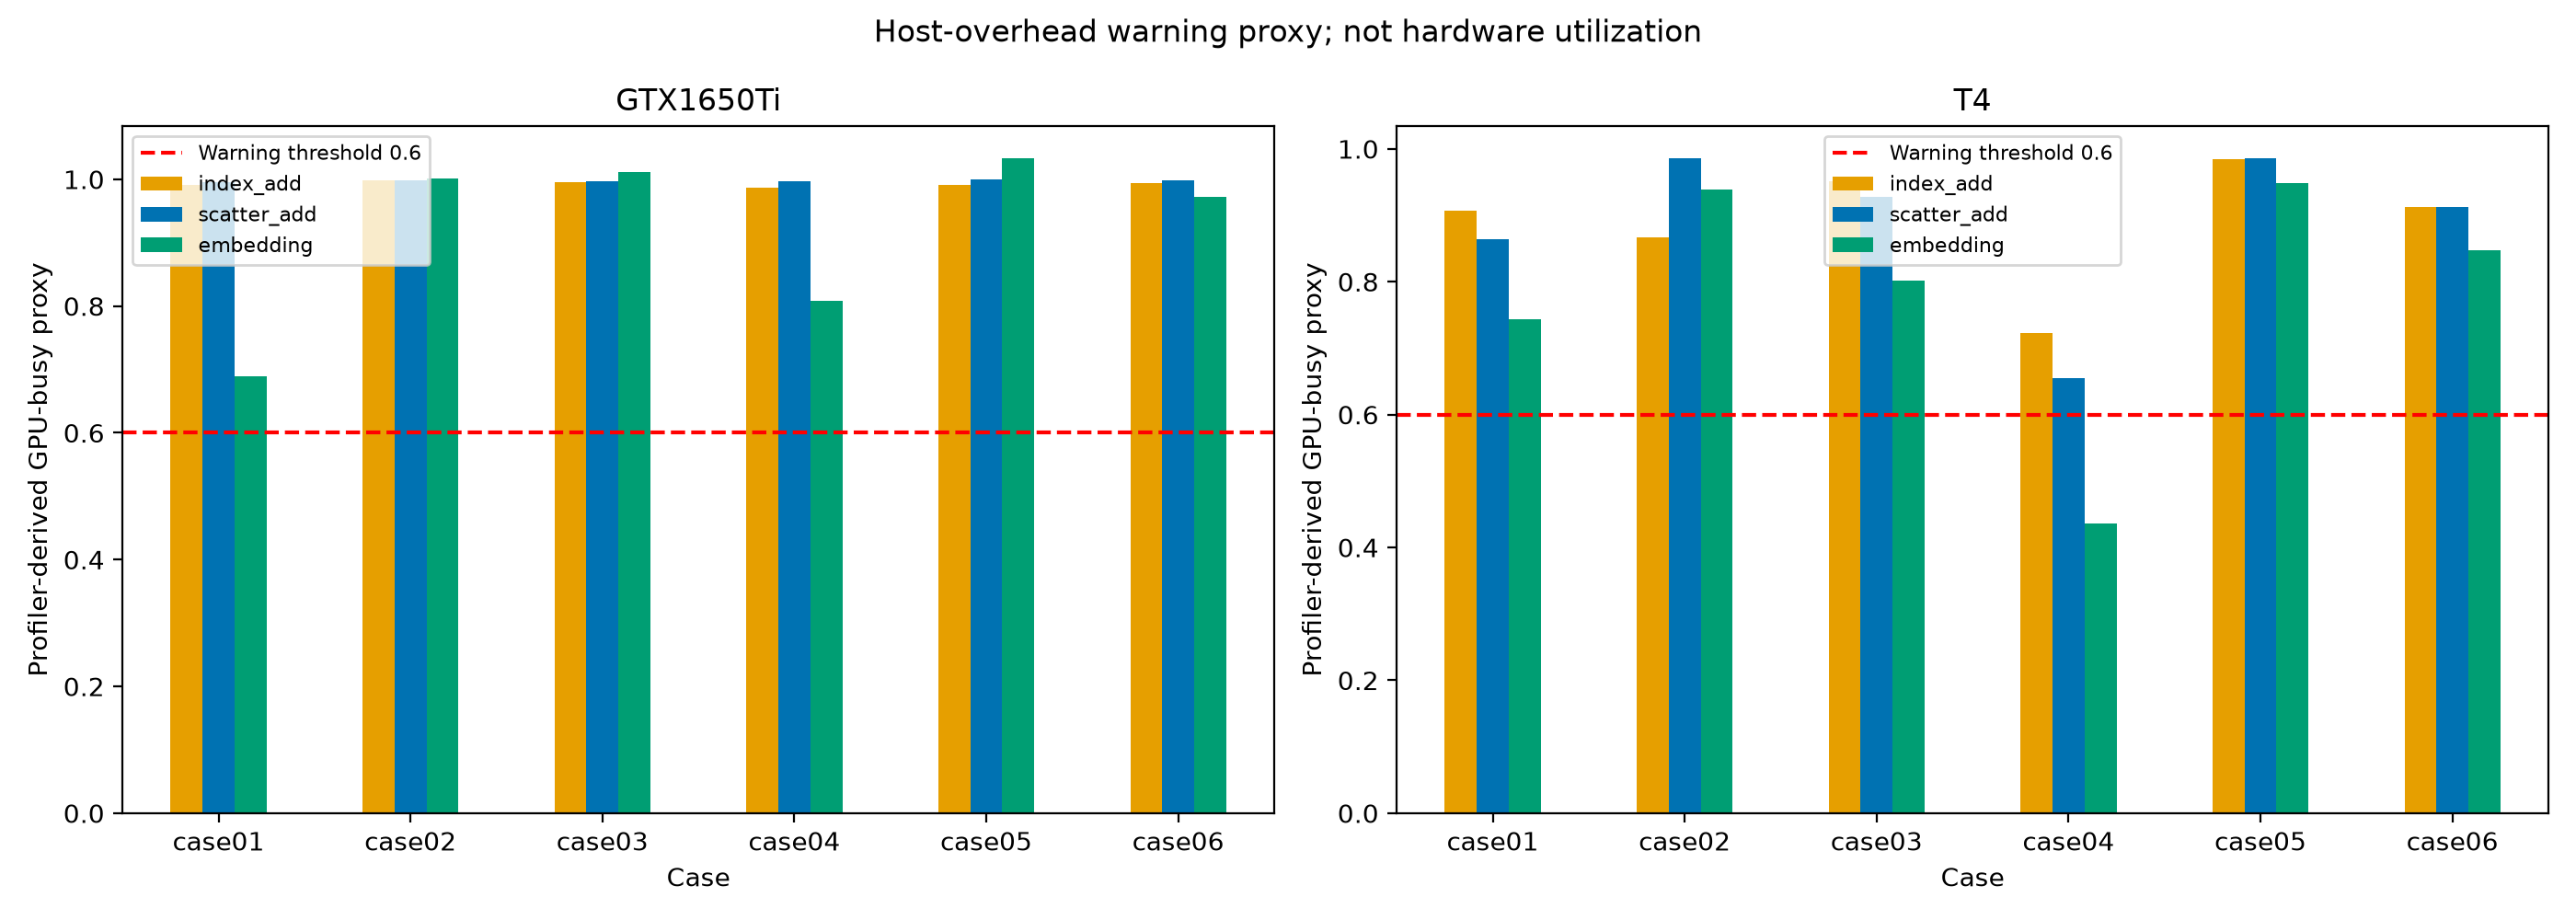
\includegraphics[width=0.80\linewidth]{figures/phase3_gpu_busy_fraction_by_case_operation.png}
\caption{Profiler-derived GPU-busy proxy by representative case and operation. The proxy is diagnostic only and is not interpreted as hardware utilization.}
\label{fig:phase3-gpu-busy}
\end{figure}

The kernel-category summary in Table~\ref{tab:phase3-kernel-category-summary} and Fig.~\ref{fig:phase3-kernel-category-share} shows that the three API paths are not merely different syntactic forms of the same CUDA behavior. The \texttt{index\_add} path is dominated by indexed accumulation kernels, the \texttt{scatter\_add} path is dominated by scatter/gather-style accumulation kernels, and the embedding backward path uses a multi-kernel composition that includes accumulation as well as sorting, scanning, or uniqueness-related components.

% Source summary: sparse-gradient/phase3_comparison_v2/phase3_kernel_category_summary.csv.
% Detailed per-case rows can be moved to an appendix or supplementary material later.
\begin{table}[tbp]
\centering
\small
\caption{Mean CUDA kernel-category shares for the representative Phase 3 profiles. Shares are averaged across the profiled cases for each environment and operation.}
\label{tab:phase3-kernel-category-summary}
\resizebox{\linewidth}{!}{%
\begin{tabular}{lllrrr}
\toprule
Environment & Operation & Dominant category & Dominant share & Secondary category & Secondary share & Other share \\
\midrule
GTX1650Ti & embedding & \texttt{embedding\_accumulate} & 0.8271 & \texttt{sort\_scan\_unique} & 0.1217 & -- \\
GTX1650Ti & \texttt{index\_add} & \texttt{index\_add\_accumulate} & 0.9677 & \texttt{zero\_fill\_memset} & 0.0323 & -- \\
GTX1650Ti & \texttt{scatter\_add} & \texttt{scatter\_add\_accumulate} & 0.9817 & \texttt{zero\_fill\_memset} & 0.0183 & -- \\
T4 & embedding & \texttt{embedding\_accumulate} & 0.6697 & \texttt{sort\_scan\_unique} & 0.2342 & 0.0347 \\
T4 & \texttt{index\_add} & \texttt{index\_add\_accumulate} & 0.9647 & \texttt{zero\_fill\_memset} & 0.0353 & -- \\
T4 & \texttt{scatter\_add} & \texttt{scatter\_add\_accumulate} & 0.9518 & \texttt{zero\_fill\_memset} & 0.0482 & -- \\
\bottomrule
\end{tabular}
}%
\end{table}


\begin{figure}[tbp]
\centering
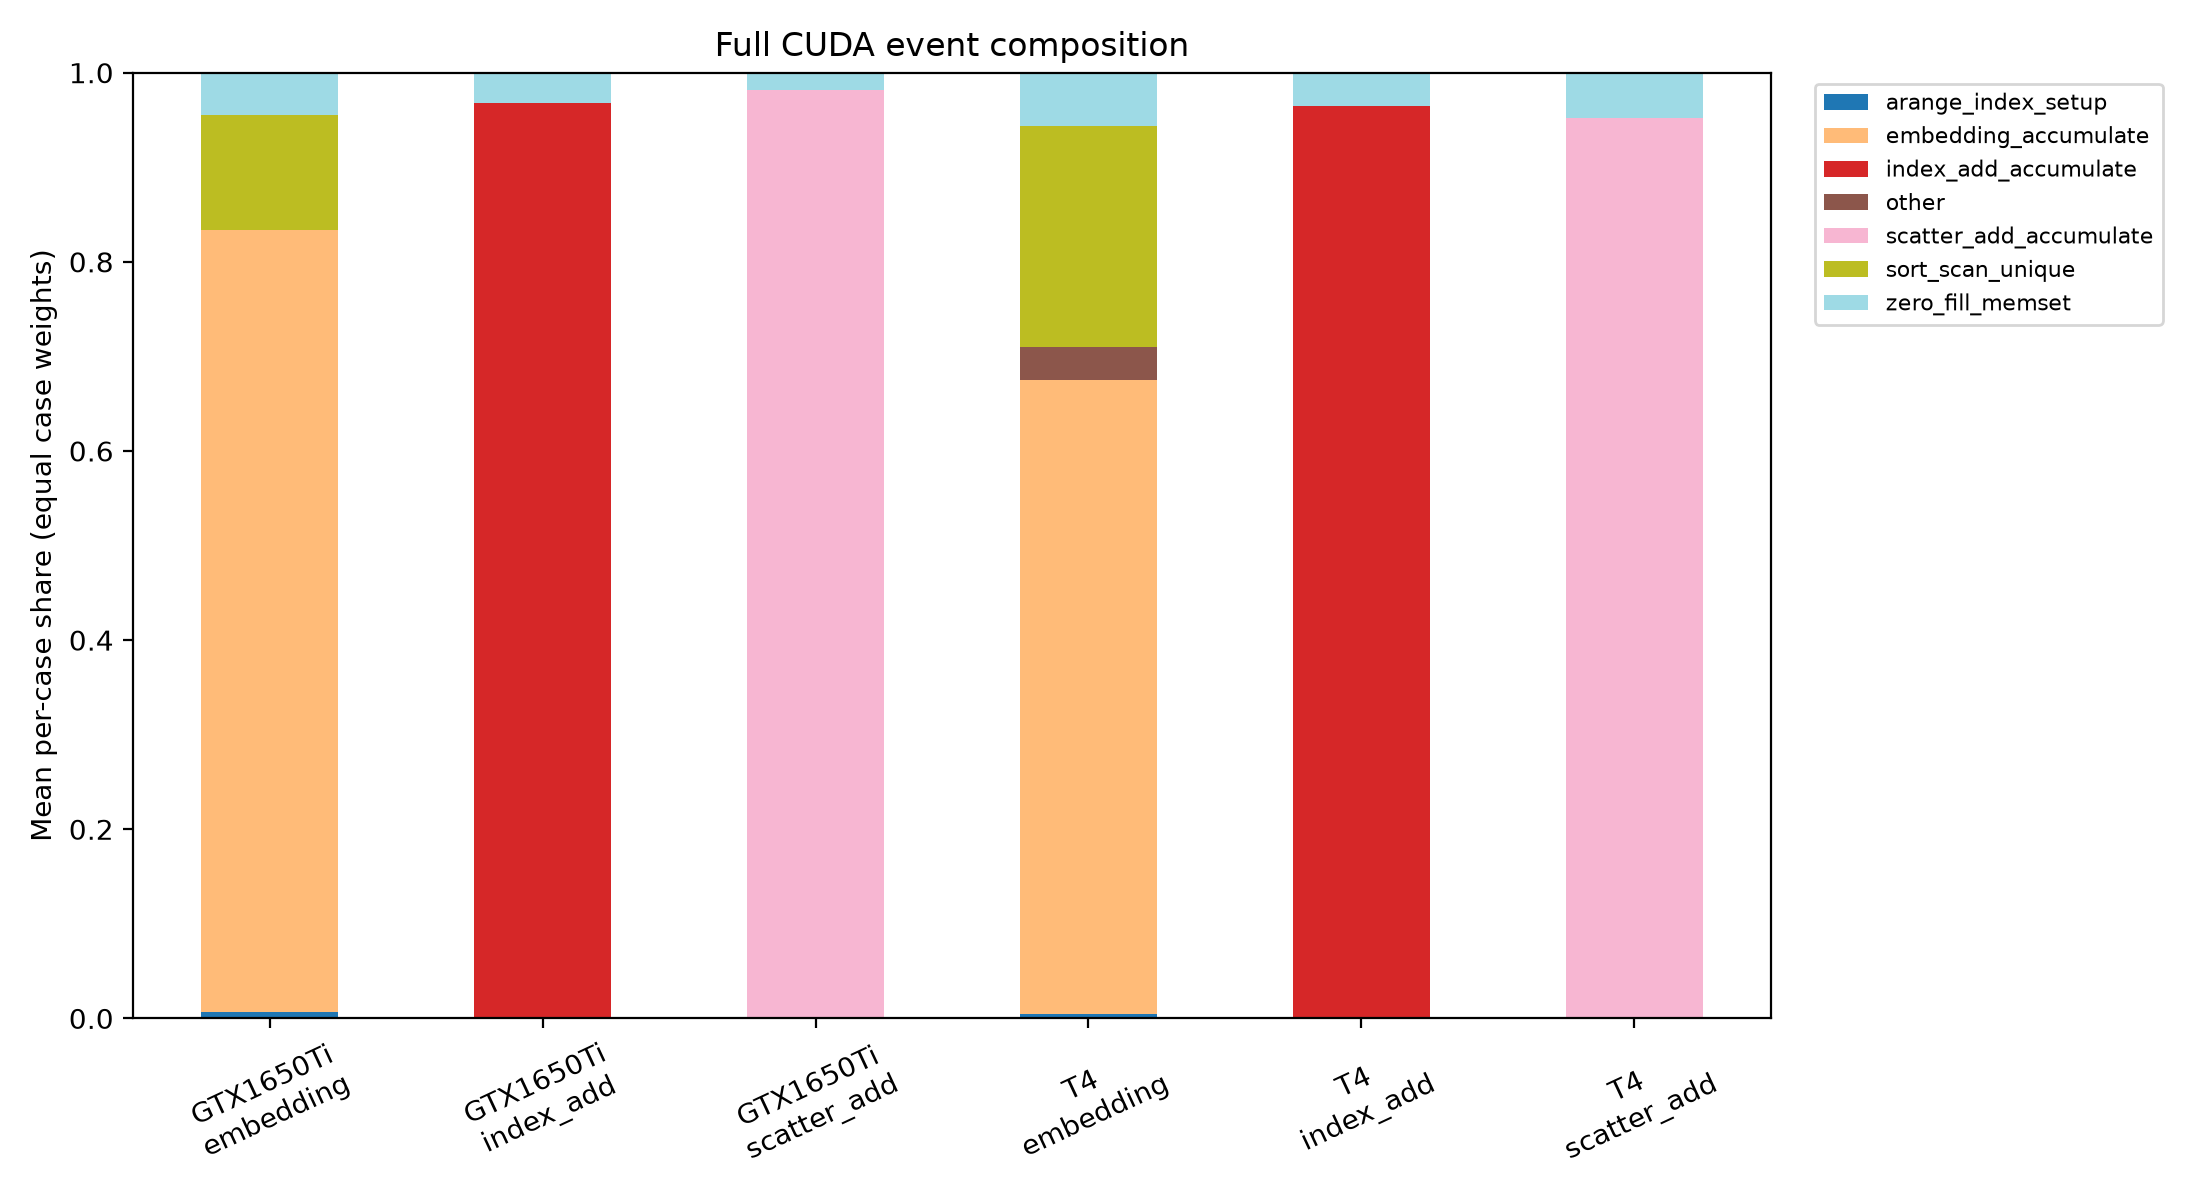
\includegraphics[width=0.80\linewidth]{figures/phase3_kernel_category_share.png}
\caption{Mean CUDA kernel-category share for the representative Phase 3 profiles. Category shares are computed from CUDA device events and summarize observed execution-path composition.}
\label{fig:phase3-kernel-category-share}
\end{figure}

The mean category shares support the intended execution-path interpretation. In both environments, \texttt{index\_add} is dominated by the \texttt{index\_add\_accumulate} category, while \texttt{scatter\_add} is dominated by the \texttt{scatter\_add\_accumulate} category. The embedding backward path is dominated by \texttt{embedding\_accumulate}, but it also contains a non-trivial \texttt{sort\_scan\_unique} component. The \texttt{other} category remains below the selected control threshold, which reduces the risk that the main attribution is hiding a large unclassified portion of CUDA time.

\subsection{Case-Level Cross-Environment Comparison}

The Phase 3 case-level comparison links the representative profiling subset to both environments and to the broader Phase 2 grid. Table~\ref{tab:phase3-case-comparison} summarizes the raw case-level winners, margins, and winner-relation categories for the six representative cases.

% Source: ../sparse-gradient/phase3_comparison_v2/phase3_case_comparison.csv
\begin{table}[tbp]
\centering
\small
\caption{Phase 3 case-level comparison across environments.}
\label{tab:phase3-case-comparison}
\resizebox{\linewidth}{!}{%
\begin{tabular}{lrrrrl}
\toprule
Case & Local winner & T4 winner & Local margin & T4 margin & Winner relation \\
\midrule
case01 & index\_add & scatter\_add & 1.670 & 1.022 & reversal near-tie \\
case02 & embedding & embedding & 2.631 & 1.706 & same decisive \\
case03 & embedding & scatter\_add & 1.116 & 1.186 & reversal decisive \\
case04 & index\_add & index\_add & 1.197 & 1.058 & same decisive \\
case05 & embedding & scatter\_add & 1.257 & 1.285 & reversal decisive \\
case06 & embedding & scatter\_add & 1.015 & 1.040 & reversal near-tie \\
\bottomrule
\end{tabular}
}%
\end{table}

Two cases provide the strongest evidence of a cross-environment reversal. In case03, the local GTX1650Ti stack selects \texttt{embedding} decisively, while the T4 stack selects \texttt{scatter\_add} decisively. In case05, the same pattern appears again: the local stack selects \texttt{embedding}, whereas the T4 stack selects \texttt{scatter\_add}. Both cases pass the stronger clean-reversal gates in the comparison analysis: they are decisively separated, have clean GPU-busy proxy status, and use exact index pairing across environments.

Fig.~\ref{fig:phase3-case-winner-comparison} visualizes the case-level winner comparison. The figure highlights that the representative subset does not support a universal ordering of APIs. Instead, it shows a mixture of agreement, near-ties, and decisive reversals.

\begin{figure}[tbp]
\centering
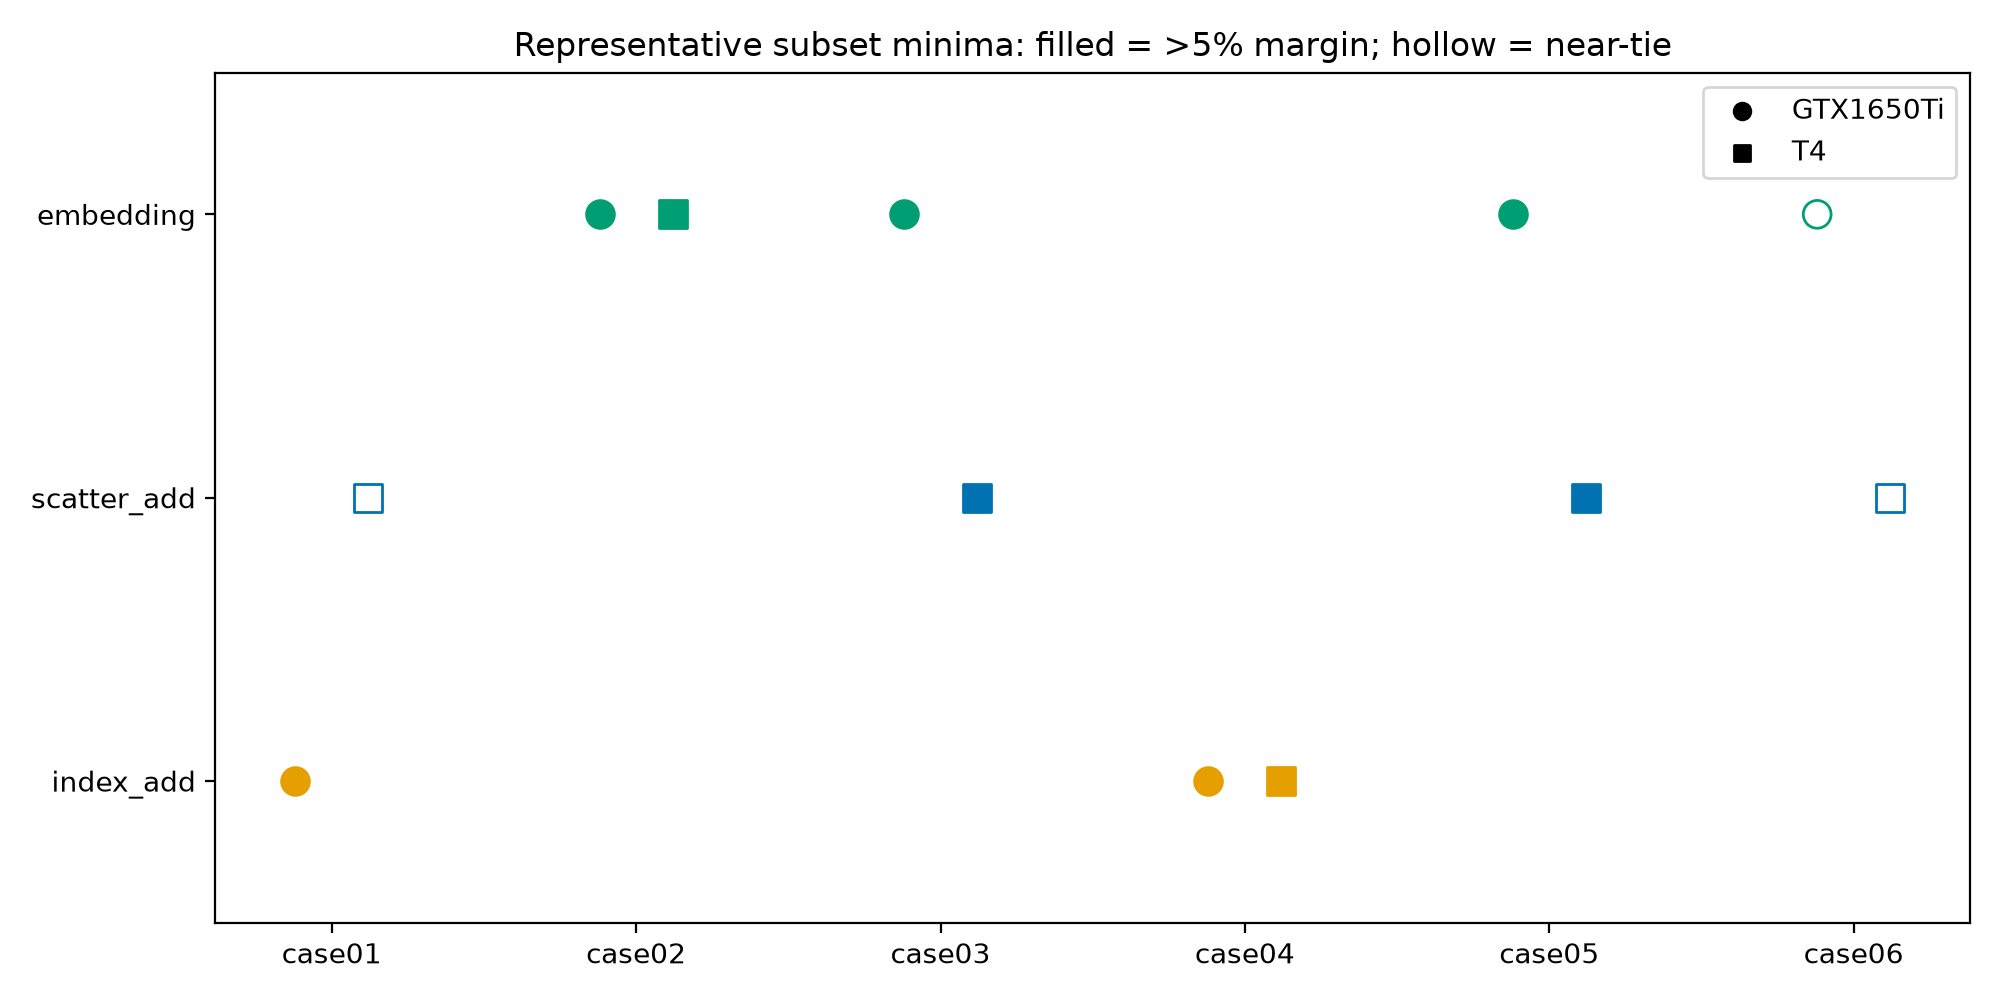
\includegraphics[width=0.80\linewidth]{figures/phase3_case_winner_comparison.png}
\caption{Representative Phase 3 winner comparison across environments. Filled markers indicate decisive practical-margin winners, while near-ties are interpreted as weak evidence.}
\label{fig:phase3-case-winner-comparison}
\end{figure}

The remaining cases serve as controls or cautionary examples. In case02, both environments select \texttt{embedding} decisively. In case04, both environments select \texttt{index\_add} decisively, although the T4 \texttt{embedding} row has a host-overhead warning and therefore prevents a fully GPU-clean claim for that case. Cases case01 and case06 exhibit different raw winners across environments, but at least one side is a near-tie, so these cases are treated as weak evidence rather than decisive reversals.

Table~\ref{tab:phase3-phase2-case-join} links the six representative Phase 3 cases back to the broader Phase 2 grid. This join is important because it verifies that the representative profiling cases are not disconnected from the main timing study. All six representative cases are present in the Phase 2 grid. The strongest reversal cases, case03 and case05, agree with the Phase 2 margin-aware winners in both environments: the local stack favors \texttt{embedding}, and the T4 stack favors \texttt{scatter\_add}. This supports the interpretation that these two profiled cases are representative examples of the broader environment-dependent behavior observed in Phase 2.

% Source: ../sparse-gradient/phase3_comparison_v2/phase3_phase2_case_join.csv
\begin{table}[tbp]
\centering
\small
\caption{Matched Phase 2 and Phase 3 case winners.}
\label{tab:phase3-phase2-case-join}
\resizebox{\linewidth}{!}{%
\begin{tabular}{lllllll}
\toprule
Case & Phase 2 local & Phase 2 T4 & Phase 2 T4 repeat & Local agree & T4 agree & Phase 3 local/T4 \\
\midrule
case01 & index\_add & tie & tie & True & False & index\_add / scatter\_add \\
case02 & embedding & embedding & embedding & True & True & embedding / embedding \\
case03 & embedding & scatter\_add & scatter\_add & True & True & embedding / scatter\_add \\
case04 & index\_add & tie & tie & True & False & index\_add / index\_add \\
case05 & embedding & scatter\_add & scatter\_add & True & True & embedding / scatter\_add \\
case06 & tie & index\_add & tie & False & False & embedding / scatter\_add \\
\bottomrule
\end{tabular}
}%
\end{table}

The case-level evidence therefore reinforces the grid-level result without replacing it. Phase 2 establishes the broader matched-performance pattern, while Phase 3 explains selected cases in terms of execution-path differences. The combination of the two phases is stronger than either alone: the timing grid shows that the fastest API changes across environments, and the profiler shows that the compared APIs exercise distinct CUDA paths.

\subsection{CUDA Path Attribution}

The claim-check table summarizes the evidence gates used to decide which result-level statements are supported by the data. These gates are included to avoid overclaiming from the representative profiling subset.

\begin{table}[tbp]
\centering
\scriptsize
\caption{Evidence gates used to avoid overclaiming from the representative Phase 3 profiling subset.}
\label{tab:phase3-claim-checks}
\resizebox{\linewidth}{!}{%
\begin{tabular}{lll}
\toprule
Check & Status & Evidence \\
\midrule
index\_add path dominance & Pass & GTX1650Ti=0.9677; T4=0.9647 \\
scatter\_add path dominance & Pass & GTX1650Ti=0.9817; T4=0.9518 \\
embedding accumulation present & Pass & GTX1650Ti=0.8271; T4=0.6697 \\
embedding sort/scan present & Pass & GTX1650Ti=0.1217; T4=0.2342 \\
other share controlled & Pass & T4/embedding=0.0347 \\
environment difference present & Pass & GTX=embedding; T4=scatter\_add \\
representative reversals present & Pass & case03, case05 \\
\bottomrule
\end{tabular}
}%
\end{table}


The path-dominance checks pass for both direct accumulation APIs. The \texttt{index\_add} path is dominated by the \texttt{index\_add\_accumulate} category in both environments, and the \texttt{scatter\_add} path is dominated by the \texttt{scatter\_add\_accumulate} category in both environments. This supports the claim that the two APIs dispatch to distinct CUDA reduction paths under the profiled workloads.

The embedding checks also pass. The embedding backward path contains a dominant accumulation component, but it also includes sorting, scanning, or uniqueness-related work. This distinguishes \texttt{Embedding.backward} from the direct \texttt{index\_add} and \texttt{scatter\_add} paths. The result is consistent with the interpretation that embedding backward is a specialized framework path rather than a simple alias for either direct accumulation API.

The claim checks also confirm that the broader Phase 2 environment-dependent pattern is present and that the representative Phase 3 subset contains strong clean reversals. In particular, case03 and case05 satisfy the strict evidence conditions: they are decisive reversals, they are not host-warning cases, they have stable timing evidence, and they use exact index pairing. These cases therefore support the paper-level statement that the relative cost of sparse-index accumulation paths can change with workload and software/hardware stack.

At the same time, the attribution remains conservative. The kernel categories are based on profiler event names and CUDA event durations, not on low-level hardware counters. Therefore, they describe observed execution paths but do not prove microarchitectural causality. The evidence supports an API-path and stack-level interpretation, not a claim that one GPU architecture alone causes the observed differences.

\subsection{Result-Level Discussion}

The combined results answer the central question of the study: standard PyTorch CUDA APIs that express related sparse-index accumulation behavior do not necessarily have interchangeable performance characteristics during backpropagation-style workloads. In the matched Phase 2 grid, the local GTX1650Ti stack most often favors the embedding backward path, whereas the T4 stacks most often favor \texttt{scatter\_add}. In the representative Phase 3 profiles, the strongest reversal cases show the same pattern at the case level: local execution favors \texttt{embedding}, while T4 execution favors \texttt{scatter\_add}.

The results also show why the difference should not be reduced to a simple API ranking. Some representative cases agree across environments, some differ only as near-ties, and two cases provide strong decisive reversals. This mixed behavior indicates that the best operation depends on workload shape, index distribution, duplicate structure, and the software/hardware stack. A recommendation such as ``always use \texttt{scatter\_add}'' or ``always use \texttt{Embedding.backward}'' would not be supported by the evidence.

The execution-path attribution provides a practical explanation for this behavior. Although the operations represent related accumulation-style computations, they dispatch to different CUDA paths. \texttt{index\_add} and \texttt{scatter\_add} use different direct accumulation kernels, while \texttt{Embedding.backward} uses a multi-kernel path that includes embedding-specific accumulation and sorting or segmentation-related work. These differences create opportunities for the relative cost of the APIs to change when the workload or execution stack changes.

For practitioners, the results suggest that sparse-gradient accumulation paths in AI training should not be selected purely from high-level API semantics. When sparse-index accumulation is a relevant part of the backward pass, especially in embedding-heavy models, recommender workloads, or other skewed-index settings, the actual execution path and target environment can materially affect performance. Microbenchmarking and profiler inspection remain useful tools for identifying which API path is most appropriate for a specific workload and deployment stack.

Finally, the results define the boundary of the present evidence. The study characterizes controlled sparse-index accumulation workloads and representative profiler cases; it does not measure full model training throughput, convergence behavior, distributed execution, or custom CUDA alternatives. Therefore, the contribution is best understood as a controlled characterization of PyTorch CUDA sparse-index gradient accumulation paths during backpropagation-style computation, rather than as a complete benchmark of AI training systems.
\section{General Discussion}
\label{sec:general-discussion}

\subsection{Significance for AI Training Workloads}

The results are significant because they address a narrow but important part of modern AI training: sparse-index accumulation during the backward pass. Many training workloads are dominated conceptually by dense linear algebra, but not all performance-critical training behavior is reducible to matrix multiplication, convolution, or attention. Models that use embedding tables, categorical features, graph-style neighborhoods, sparse identifiers, or irregular index references often include operations in which many source vectors must be accumulated into a dense parameter-gradient structure \cite{gupta2020architectural,pytorchStableEmbedding}. In these cases, the performance of the backward pass can depend strongly on indexed accumulation behavior.

This study shows that high-level API similarity is not sufficient to infer equivalent CUDA behavior. The compared operations express related accumulation-style computations, but the profiling evidence shows that they dispatch to different CUDA execution paths \cite{pytorchStableIndexAdd,pytorchStableScatterAdd,pytorchStableEmbedding}. This matters for AI training because practitioners often choose between framework APIs based on readability, convenience, or semantic equivalence at the tensor-programming level. The results suggest that such choices can also affect the actual training-time cost of sparse-gradient accumulation.

The finding is especially relevant for embedding-heavy models. In recommender systems, natural language systems with large token embeddings, graph neural networks, and other sparse-feature models, embedding tables transform sparse identifiers into dense vectors during the forward pass and require gradient accumulation during the backward pass \cite{acun2021training,nvidia_recsys_best_practices,pytorchStableEmbedding}. The backward phase is therefore not merely an implementation detail; it is part of the training workload that can interact with index duplication, skewed access patterns, and framework-level kernel dispatch.

The database analogy that motivated this work is also useful for interpretation. Sparse-index gradient accumulation resembles a grouped update or indexed aggregation: many input records reference a smaller set of destination rows, and repeated keys must be accumulated. In database systems, the cost of such an operation depends on key distribution, skew, memory layout, grouping strategy, and execution engine. The same conceptual issue appears in AI training workloads: index distributions such as uniform, Zipf, and hotspot patterns can change the relative cost of the accumulation path. This connection helps explain why a single universal API ranking is unlikely to be robust across workloads.

\subsection{Practical Implications}

The most direct practical implication is that sparse-gradient accumulation paths should be benchmarked under the intended workload and execution stack. The results do not support a universal recommendation such as always using \texttt{index\_add}, always using \texttt{scatter\_add}, or always relying on \texttt{Embedding.backward}. Instead, the fastest path depends on the workload shape, duplicate-index structure, feature dimension, and software/hardware environment.

For practitioners, this means that API selection should be treated as an empirical systems decision when sparse-index accumulation is performance-relevant. If a model spends a meaningful fraction of training time in embedding backward, scatter/reduce operations, or indexed accumulation kernels, then small focused benchmarks can be useful before finalizing an implementation \cite{pytorchStableEmbedding,pytorchStableIndexAdd,pytorchStableScatterAdd}. A benchmark does not need to reproduce a full production model in order to be useful, but it should reproduce the important dimensions of the sparse operation: row count, number of indices, feature dimension, index skew, duplicate frequency, and target hardware/software stack.

The results also suggest that profiler inspection should accompany timing measurements. Timing alone can show that one path is faster, but it cannot explain whether two APIs use similar or different execution paths. In this study, the profiler results show that \texttt{index\_add}, \texttt{scatter\_add}, and \texttt{Embedding.backward} rely on different CUDA kernel compositions. This kind of evidence is useful when deciding whether an observed timing difference is likely to be a minor measurement artifact or a consequence of different execution mechanisms.

Another implication concerns framework upgrades and deployment portability. Since the observed behavior is interpreted at the stack level, changes in PyTorch version, CUDA version, driver, GPU type, or hosted runtime may change the relative behavior of the same high-level code. A training implementation that is fastest on one environment may not remain fastest after moving to another GPU, another CUDA version, or another PyTorch release. This is particularly important for workflows that prototype locally and later train in cloud environments.

Finally, the results encourage a cautious interpretation of abstraction in ML frameworks. High-level tensor APIs are designed to improve productivity and correctness, but performance-critical training code may still depend on lower-level dispatch decisions. This does not mean that practitioners should avoid high-level APIs. Rather, it means that when the sparse backward path becomes a bottleneck, API-level alternatives should be evaluated as concrete execution paths rather than only as mathematical expressions.

\subsection{Limitations}

The study has several limitations. First, the experiments focus on controlled sparse-index accumulation workloads rather than complete model training. This design is intentional because it isolates the accumulation behavior, but it also means that the results do not directly measure end-to-end training throughput, convergence time, validation accuracy, optimizer overhead, data loading, distributed communication, or model-level scheduling effects.

Second, the profiling phase uses a representative subset of cases rather than the full matched workload grid. The representative cases are useful for understanding execution-path differences, but they should not be interpreted as a statistically complete sample of all possible sparse-gradient workloads. The main grid-level timing evidence comes from Phase 2, while Phase 3 provides attribution for selected cases.

Third, the cross-environment comparison is a stack-level comparison, not an isolated hardware experiment. The local GTX1650Ti and T4 environments differ in GPU model, operating system, PyTorch version, CUDA version, and runtime conditions. Therefore, the study cannot claim that the GPU architecture alone caused the observed differences. The correct interpretation is that the relative cost of the API paths changes across combined hardware/software stacks.

Fourth, the profiler attribution is based on PyTorch profiler events and CUDA kernel names, not on lower-level hardware counters. This is sufficient for identifying distinct execution paths, but it does not fully explain the microarchitectural causes of the observed timing differences. The study does not use Nsight Compute counters, warp-level metrics, memory-transaction analysis, occupancy analysis, or cache-behavior counters.

Fifth, the study evaluates standard PyTorch CUDA paths rather than custom CUDA implementations or specialized embedding-training libraries \cite{pytorchStableEmbedding,pytorchStableIndexAdd,pytorchStableScatterAdd,nvidia_recsys_best_practices}. This scope is appropriate for understanding what practitioners obtain from common PyTorch APIs, but it does not establish the best possible performance attainable for sparse-index accumulation. A custom fused implementation or a specialized recommender-system training framework could produce different results.

Sixth, the workloads are synthetic and controlled. Although the uniform, Zipf, and hotspot distributions capture important access-pattern properties, they do not fully reproduce all characteristics of real training datasets. Real systems may include multiple embedding tables, mixed feature widths, optimizer state updates, sharding, caching, distributed all-to-all communication, and model-specific preprocessing. The results should therefore be interpreted as controlled evidence about a core sparse-gradient mechanism, not as a complete simulation of production training.

\subsection{Generalizability}

The results generalize most directly to PyTorch CUDA workloads that perform dense sparse-index accumulation during backpropagation or backward-like computations. The strongest connection is to embedding-heavy models and other workloads where repeated indices accumulate contributions into rows of a parameter-gradient tensor. This includes recommender-style models, categorical-feature models, graph workloads with repeated destination nodes, and other training procedures that use scatter/reduce-like updates \cite{acun2021training,nvidia_recsys_best_practices}.

The results should generalize conceptually, but not numerically, to other frameworks and hardware stacks. The conceptual lesson is that equivalent or related high-level operations may dispatch to different backend execution paths, and those paths may respond differently to skew, duplication, feature dimension, and memory layout. However, the specific winner counts and timing margins reported in this study are tied to the tested PyTorch, CUDA, and GPU environments. Other frameworks, compiler backends, GPU architectures, or library versions may expose different behavior.

The database analogy also supports generalization at the level of systems reasoning. Sparse-gradient accumulation can be viewed as a form of indexed aggregation over repeated keys. Systems that process such patterns must handle skew, duplicate destinations, memory contention, and reduction order. These issues are not unique to PyTorch or to the exact APIs studied here. They are broader properties of irregular aggregation workloads. Therefore, the paper's main generalizable claim is not that a specific PyTorch API is always preferable, but that sparse-index accumulation should be treated as a workload- and stack-dependent systems problem.

At the same time, the results should not be generalized to all AI training workloads. Dense transformer training, convolution-heavy vision models, and dense MLP workloads may be dominated by matrix multiplication or convolution kernels rather than sparse-index accumulation. In such settings, the API paths studied here may contribute little or nothing to total training time. The practical relevance of the findings depends on whether indexed gradient accumulation is a meaningful component of the model's backward pass.

\subsection{Future Work}

Future work should extend the study from controlled sparse-index accumulation kernels to small end-to-end training proxies. A natural next step is an embedding-heavy training step consisting of an embedding lookup, pooling or reduction, a small prediction head, a loss function, and a backward pass \cite{gupta2020architectural,pytorchStableEmbedding}. Such an experiment would help determine how much of the isolated accumulation behavior remains visible when embedded in a complete autograd graph. It should still be treated carefully, because end-to-end timing would include additional overhead from forward computation, loss evaluation, optimizer updates, and framework scheduling.

A second direction is to evaluate additional hardware and software stacks. The present study compares a local GTX1650Ti stack and a T4 stack, but the same benchmark protocol could be applied to newer NVIDIA GPUs, data-center GPUs, consumer GPUs, and different PyTorch/CUDA combinations. This would help determine whether the observed stack-dependent behavior is common across generations or specific to the tested environments.

A third direction is to add lower-level profiling. Nsight Compute metrics could be used to investigate memory throughput, atomic behavior, occupancy, warp divergence, cache behavior, and memory-transaction efficiency. These metrics would make it possible to move from execution-path attribution toward a deeper microarchitectural explanation of why particular APIs win under particular workload shapes.

A fourth direction is to evaluate sparse optimizer behavior and sparse-gradient modes more directly. PyTorch embedding layers can optionally produce sparse gradients, and optimizers differ in their support for sparse gradient representations \cite{pytorchStableEmbedding}. Comparing dense-gradient accumulation, sparse-gradient accumulation, and optimizer update cost would connect the present study more directly to full training systems.

A fifth direction is to relate synthetic index distributions to real datasets. The current workload design includes uniform, Zipf, and hotspot patterns, but production recommender and graph workloads may exhibit more complex temporal locality, feature co-occurrence, and table-specific skew. Replaying real or trace-derived index distributions would improve external validity while preserving the controlled methodology developed here.

Finally, future work could compare standard PyTorch APIs with custom fused kernels or specialized recommender-system libraries. This would answer a different question from the present paper. The current study asks how common PyTorch CUDA paths behave under controlled sparse-gradient accumulation workloads. A follow-up study could ask how close these standard paths are to optimized custom implementations and whether API-level performance gaps can be reduced through fusion, sorting, deduplication, or workload-aware scheduling.

\section{Conclusion}
\label{sec:conclusion}

This paper presented a controlled empirical study of sparse-index gradient accumulation during backpropagation-style AI training workloads. The study focused on standard PyTorch CUDA paths, specifically \texttt{index\_add}, \texttt{scatter\_add}, and \texttt{Embedding.backward}, rather than custom CUDA kernels or full end-to-end model training. The objective was to determine whether these high-level APIs exhibit interchangeable performance behavior under matched sparse-index accumulation workloads, and to relate the observed timing differences to CUDA execution-path evidence.

The results show that high-level API similarity does not imply equivalent CUDA behavior. In the matched benchmark phase, the fastest operation depended on the workload and execution stack. The local GTX1650Ti stack most often favored the embedding backward path, whereas the T4 stacks most often favored \texttt{scatter\_add} under the practical-margin rule. The representative profiling phase further showed that the compared APIs dispatch to distinct CUDA kernel compositions. The \texttt{index\_add} path was dominated by indexed accumulation kernels, the \texttt{scatter\_add} path by scatter/gather-style accumulation kernels, and \texttt{Embedding.backward} by a multi-kernel backward path that included accumulation as well as sorting or segmentation-related components.

These findings support the main conclusion that sparse-index gradient accumulation should be treated as a workload- and stack-dependent systems problem. For embedding-heavy models, recommender-style workloads, graph-like aggregation patterns, and other sparse-feature training settings, selecting an accumulation path only from high-level tensor semantics can be misleading. Focused benchmarking and profiler inspection are useful when indexed gradient accumulation contributes meaningfully to training cost.

The study also defines clear boundaries for this conclusion. The experiments characterize controlled sparse-index accumulation workloads and representative profiling cases; they do not establish a universal fastest PyTorch API, an isolated hardware-causal explanation, or end-to-end training throughput for complete models. The cross-environment comparison is interpreted at the combined hardware/software stack level, since GPU model, operating system, PyTorch version, CUDA version, and runtime conditions differ together.

Future work should extend this characterization to additional GPU generations, PyTorch/CUDA releases, and embedding-heavy training proxies. A natural next step is to evaluate whether the isolated accumulation behavior observed here remains visible inside a complete training step that includes embedding lookup, pooling or feature interaction, a prediction head, loss computation, backward propagation, and optimizer updates. Lower-level profiling with hardware counters could also help explain the microarchitectural causes behind the observed API-dependent behavior.

\section*{Acknowledgements}
The authors declare no specific funding or personal acknowledgements for this working manuscript.

\section*{Competing interests}
The authors declare that they have no competing interests or financial conflicts to disclose.

\bibliographystyle{fcs}
\bibliography{ref}

\end{document}
